\chapter{SYSTEM ANALYSIS AND DESIGN}
\section{System Analysis}
The project is following a structured approach that utilizes the Rapid Application Development (RAD) methodology. This approach segments the project into smaller, manageable components, allowing for incremental progress through iterative development. Individual modules are developed and integrated progressively, focusing on delivering and refining smaller segments. This method ensures continuous improvement and alignment with the overall goals while effectively managing the project through ongoing feedback and adjustments.
\subsection{Requirement Analysis}
Requirement analysis is a critical phase in the software development lifecycle that focuses on understanding and documenting the needs and expectations of stakeholders. This process involves gathering detailed information about what users require from a system, which includes identifying functional requirements (what the system should do), non-functional requirements (how the system should perform), and constraints (limitations or restrictions). The goal is to create a comprehensive and clear specification that guides the development team in designing and implementing the system. Effective requirement analysis ensures that the final product aligns with user needs and business objectives, reduces the risk of project failure, and facilitates efficient communication among stakeholders. By thoroughly analyzing requirements, teams can address potential issues early, prioritize features, and ensure a smoother development process.
\subsubsection{Functional Requirements}The functional requirements of LabXplorerX are mentioned below:
\begin{itemize}
    \item \textbf{User Profiles and Progress Tracking:} LabXplorerX enables children and teachers to create personalized profiles for tracking their learning progress and achievements. Users can log in with unique credentials, update their profiles with educational interests and avatars, and monitor their completion of simulations and quizzes. The progress tracking feature records tasks completed, concepts learned, and achievements unlocked, offering a comprehensive view of individual learning journeys and performance over time.

    \item \textbf{Interactive Virtual Simulations:} LabXplorerX offers a range of interactive virtual simulations, including Basic Electronics, Basic Chemistry, Basic Astronomy, and an Online Coding Environment. These simulations provide immersive experiences where users can engage in hands-on activities, such as manipulating virtual equipment and conducting experiments. By integrating interactive animations and real-world scenarios, LabXplorerX facilitates experiential learning, allowing users to explore scientific principles and phenomena in a dynamic digital environment.

    \item \textbf{Capsule Tools: } Creators are equipped with specialized tools to create and manage educational capsules and assign tasks to students. They can design experiment capsules with sequential steps, interactive quizzes, and checkpoints to assess student progress. Teachers review completed assignments, provide feedback, and evaluate learning outcomes, ensuring that learning experiences are tailored to individual needs. Learning capsules, similar to capsules or blog entries, provide focused content and insights on specific topics, allowing for an organized and structured approach to content delivery and knowledge reinforcement.

    \item \textbf{Discussion section for Learning Capsules:} LabXplorerX includes a discussion section that promotes collaborative learning and knowledge sharing. Both students and teachers can start discussions, ask questions, share insights, and respond to others' posts. The section supports threaded discussions, tagging, and search functionalities, fostering meaningful interactions and peer engagement within the learning community.

    \item \textbf{Quizzes and Learning Capsules:} LabXplorerX integrates quizzes and learning capsules to reinforce knowledge and assess comprehension. Quizzes are designed to evaluate understanding of concepts covered in simulations, while learning capsules provide bite-sized, focused content on specific topics. These features help consolidate learning and provide instant feedback.

    \item \textbf{Admin Dashboard:} The admin dashboard in LabXplorerX offers a centralized interface for managing user accounts, monitoring platform usage, and overseeing system performance. Administrators can access detailed analytics, configure system settings, and manage content to ensure smooth operation and address any issues that arise.
\end{itemize}

\subsubsection{Nonfunctional Requirements}
The nonfunctional requirements of LabXplorerX are mentioned below:
\begin{itemize}
    \item \textbf{Performance Enhancement:} The focus on performance involves optimizing the platform to handle high user loads and complex simulations efficiently. This includes minimizing reliance on external frameworks and ensuring smooth and responsive interactions.
    \item \textbf{Authentication Security:} Security is a paramount concern. To enhance the platform’s security, advanced authentication algorithms, particularly focusing on hashing techniques within the backend environment, have been implemented. This ensures that user authentication data is stored and managed in a highly secure manner.
    \item \textbf{Better UX Design:} User experience is central to the project’s success. The emphasis on better UX design means that every aspect of the platform’s interface, from navigation to interaction, will be meticulously crafted to ensure a seamless and intuitive experience. This design approach caters not only to experienced users but also to newcomers, ensuring that all users can effortlessly navigate and engage with the platform.
    \item \textbf{Responsive Design:} Recognizing the diverse range of devices and browsers that users utilize, the creation of a responsive design is important for this project. This means that the platform’s design and functionality will adapt flawlessly to various screen sizes, ensuring that users can access and interact with the platform effectively, whether they are using a desktop computer, tablet, or smartphone. This responsiveness guarantees a consistent and satisfying experience aweb different devices and platforms, promoting accessibility and usability.
\end{itemize}
\section{Feasibility Analysis}
A feasibility study is a systematic and structured analysis conducted to determine the viability and practicality of a proposed project plan. It serves as an evaluation tool to assess whether the project can be successfully implemented and if it aligns with the organization's goals and objectives. It involves gathering and analyzing relevant information to determine if the project is technically feasible, operationally feasible, economically feasible, and scheduling feasible.
\subsection{Economical Feasibility}
The development of the web application will utilize a range of free and open-source software development tools. For the frontend, React, a popular JavaScript library for building dynamic and interactive user interfaces, will be used. On the backend, Express, a minimal and flexible Node.js web application framework, will handle server-side logic and HTTP requests. PostgreSQL, an open-source relational database management system known for its reliability and performance, will be employed for database management. Interactive simulations will be created using Phaser, a robust HTML5 game framework, while Unity, a powerful cross-platform game engine, will be used for more complex simulations and 3D elements. Additionally, funds will be allocated for economical server hosting to ensure the application remains accessible to users while managing costs effectively.
\subsection{Operational Feasibility}
LabXplorerX prioritizes operational feasibility through a user-centric design approach, emphasizing simplicity and ease of use. The system is highly interactive, enabling both students and educators to navigate effortlessly without requiring extensive technical knowledge. The user interface (UI) features a clean layout and intuitive controls, ensuring a seamless experience when accessing virtual environments and educational resources. By minimizing the need for extensive training and reducing potential barriers to adoption, LabXplorerX enhances user acceptance and engagement. The straightforward design promotes effective use of the app's features, supports educational activities, and fosters a positive user experience.
\subsection{Technical Feasibility}
Combining Express.js with React and PostgreSQL offers a robust and scalable solution for developing modern applications. Express.js, built on Node.js, provides an efficient backend framework for creating RESTful APIs and managing server-side logic. PostgreSQL, known for its reliability and advanced data management features, serves as a solid foundation for secure and efficient data storage and querying. On the frontend, React facilitates the creation of responsive and visually appealing applications across multiple platforms using a single codebase. This stack leverages the strengths of each technology: Express.js for backend scalability and API development, PostgreSQL for comprehensive data handling, and React for seamless and dynamic UI development. Supported by active communities and extensive documentation, this combination ensures ample technical support, resources, and flexibility for both deployment and maintenance, making it an ideal choice for delivering modern, interactive applications.
\section{Structured System Modelling }
Structured system modeling is a methodical approach used to design complex systems by decomposing them into manageable components and utilizing formal diagrams and tools. This approach aids in clearly defining system requirements, workflows, and interactions. By breaking down a system into its constituent parts, structured system modeling facilitates a thorough understanding of its structure and behavior. The use of formal diagrams and tools ensures that all aspects of the system are documented and analyzed systematically, which enhances clarity, communication, and accuracy throughout the design process. This methodical approach supports the creation of well-organized and efficient systems, improving overall design quality and project outcomes.
\newpage
\subsection{Process Modeling: DFD}
Processing Modeling Data Flow Diagrams (DFDs) visually represent the flow of data within a system, showing how inputs are processed into outputs. They help in understanding the system's functionality and data movement, aiding in the design and analysis of processes.
\begin{figure}[H]
    \centering
    \rotatebox{90}{
        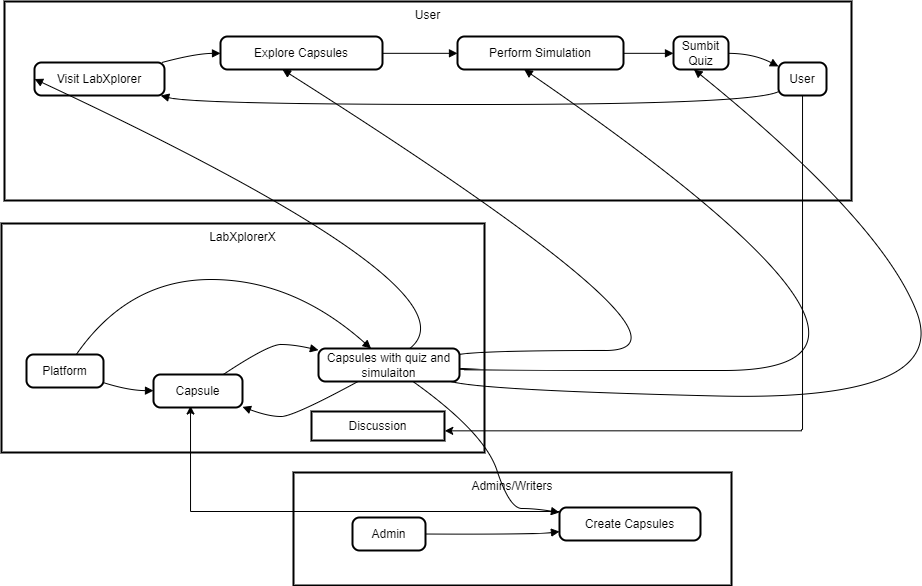
\includegraphics[height = 12cm]{Diagrams/DFD.drawio.png}
    }
    \caption{Process Model: Logical DFD}
\end{figure}
\newpage
\newpage
\subsection{Data Modelling(ER-Diagram)}
The Entity-Relationship (ER) Diagram is primarily used to design a database schema. The ER diagram provided below facilitates the creation of a database in SQL by clearly illustrating the entities, their attributes, and the relationships between them. This visual representation helps in structuring the database effectively, ensuring that all necessary data elements and their interconnections are accounted for.
\section*{Entities and Attributes}
\begin{itemize}
    \item \textbf{Users}
    \begin{itemize}
        \item \texttt{id}: Unique identifier for the user.
        \item \texttt{username}: The name of the user.
        \item \texttt{email}: Email of the user.
        \item \texttt{password}: Password for user authentication.
        \item \texttt{email\_verification\_token}: Token to verify the email.
        \item \texttt{email\_verified}: Status indicating whether the user's email is verified.
    \end{itemize}
    
    \item \textbf{Capsules}
    \begin{itemize}
        \item \texttt{id}: Unique identifier for the capsule.
        \item \texttt{title}: Title of the capsule.
        \item \texttt{description}: Description of the capsule.
        \item \texttt{thumbnail}: Image representing the capsule.
        \item \texttt{images}: Additional images related to the capsule.
        \item \texttt{pdf}: PDF documents associated with the capsule.
        \item \texttt{category}: The category to which the capsule belongs.
        \item \texttt{author\_id}: Reference to the user who created the capsule.
    \end{itemize}
    
    \item \textbf{Simulations}
    \begin{itemize}
        \item \texttt{id}: Unique identifier for the simulation.
        \item \texttt{title}: Title of the simulation.
        \item \texttt{description}: Description of the simulation.
        \item \texttt{link}: URL or reference to the simulation.
        \item \texttt{category}: The category of the simulation.
    \end{itemize}
    
    \item \textbf{Comments}
    \begin{itemize}
        \item \texttt{comment\_id}: Unique identifier for the comment.
        \item \texttt{comment\_text}: The text of the comment.
        \item \texttt{user\_id}: Reference to the user who made the comment.
        \item \texttt{capsule\_id}: Reference to the capsule that was commented on.
    \end{itemize}
    
    \item \textbf{Quiz}
    \begin{itemize}
        \item \texttt{quiz\_id}: Unique identifier for the quiz.
        \item \texttt{title}: Title of the quiz.
        \item \texttt{category}: The category of the quiz.
        \item \texttt{capsule\_id}: Reference to the capsule related to the quiz.
    \end{itemize}
    \item \textbf{Options}
    \begin{itemize}
        \item \texttt{option\_id}: Unique identifier for the option.
        \item \texttt{option\_text}: Text of the quiz option.
        \item \texttt{is\_correct}: Boolean indicating if the option is correct.
        \item \texttt{quiz\_id}: Reference to the quiz.
    \end{itemize}
    
    \item \textbf{Favorites}
    \begin{itemize}
        \item \texttt{user\_id}: Reference to the user.
        \item \texttt{capsule\_id}: Reference to the capsule marked as a favorite.
    \end{itemize}
\end{itemize}
\begin{figure}[H]
    \centering
    \rotatebox{90}{
        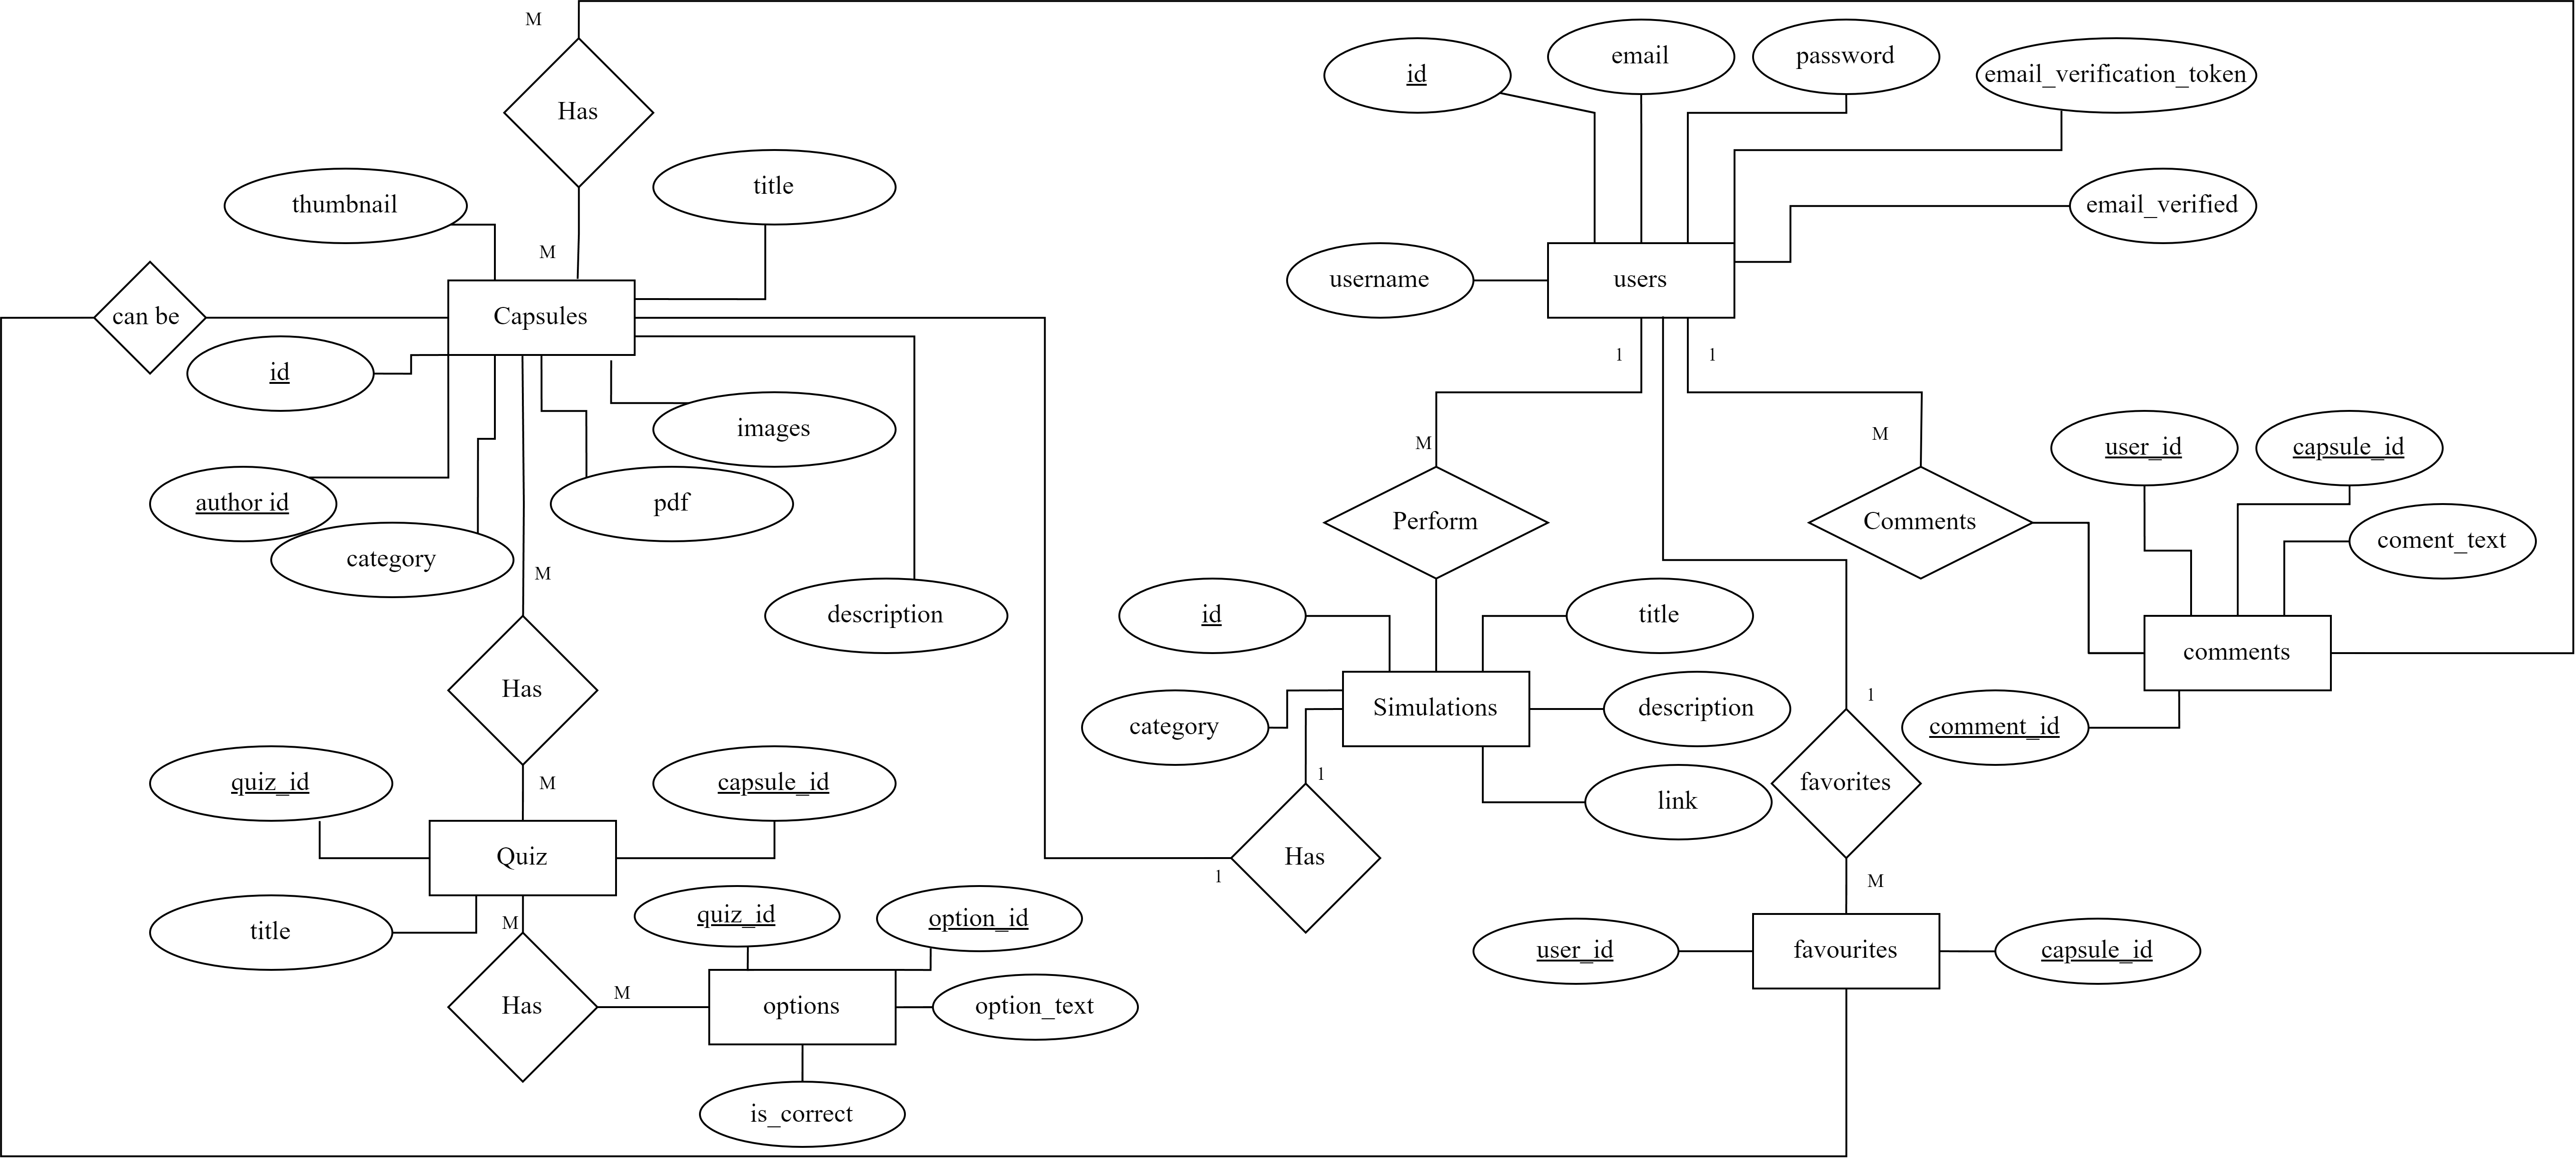
\includegraphics[height=10.5cm]{Diagrams/er.drawio.png}
    }
    \caption{ER Diagram of System Data}
\end{figure}
\newpage
\section{Structured System Design}
\subsection{Architecture Design}
The following diagram illustrates the architecture of our application. The application is structured using a three-tier architecture to ensure a clear separation of concerns and efficient functionality. The Presentation Layer, built with React.js, manages the user interface and user interactions. The Business Logic Layer, developed with Node.js and Express, handles core operations through middleware, routes, models, controllers, and utilities. Finally, the Data Management Layer uses PostgreSQL for relational database management and local server storage for handling files.
\begin{figure}[H]
    \centering
    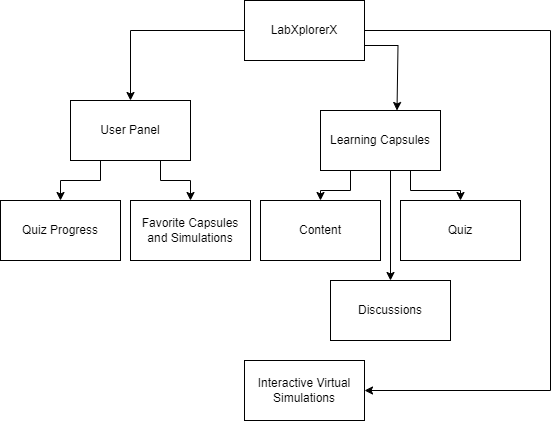
\includegraphics[height=16cm]{Diagrams/Main_Block.png}
    \caption{Three Tier Architecture of System}
\end{figure}

\newpage
\subsection{Database Schema Design}
The schema design details the tables, their attributes, and the relationships between them, ensuring that data is stored efficiently and consistently. This design includes defining primary keys to uniquely identify records, foreign keys to establish relationships between tables, and constraints to maintain data integrity. The schema design provides a clear blueprint for creating and managing the database, supporting effective data organization and retrieval as per the application’s requirements.
\begin{figure}[H]
   \centering
    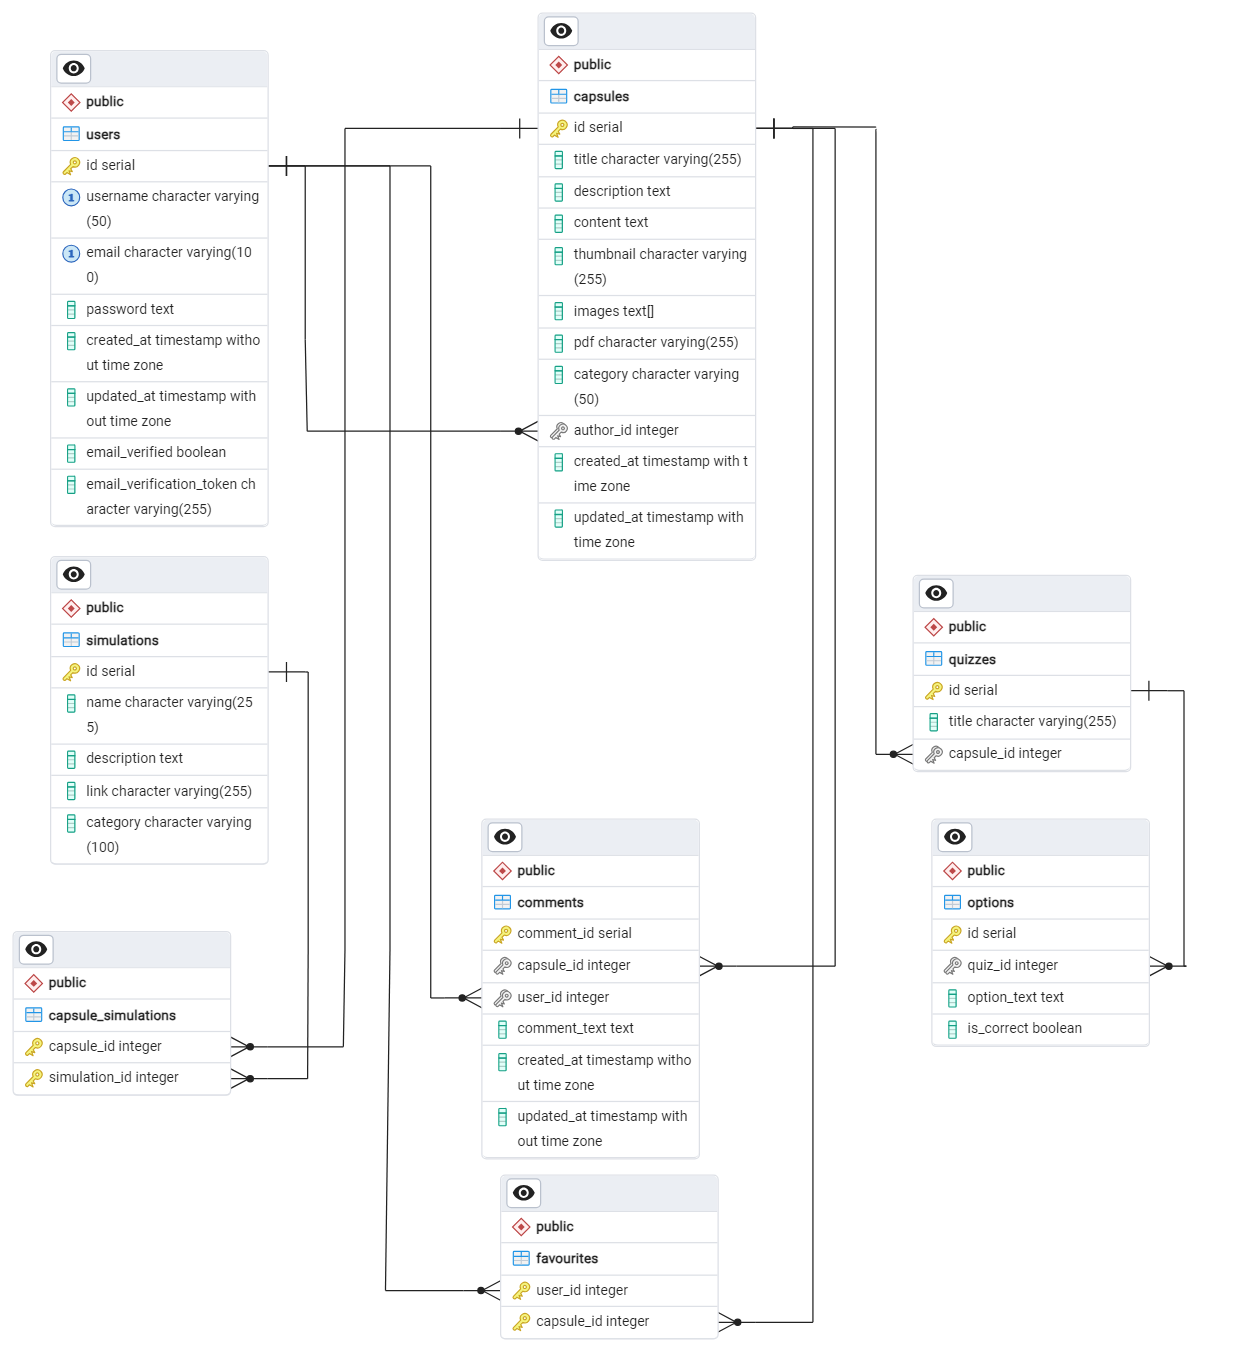
\includegraphics[height = 17cm]{Diagrams/Schema Design.png}
    \caption{Schema Design}
\end{figure}
\newpage

\subsection{Interface Design}
Here are the UI/UX Designs created for this project:
\begin{figure}[H]
   \centering
    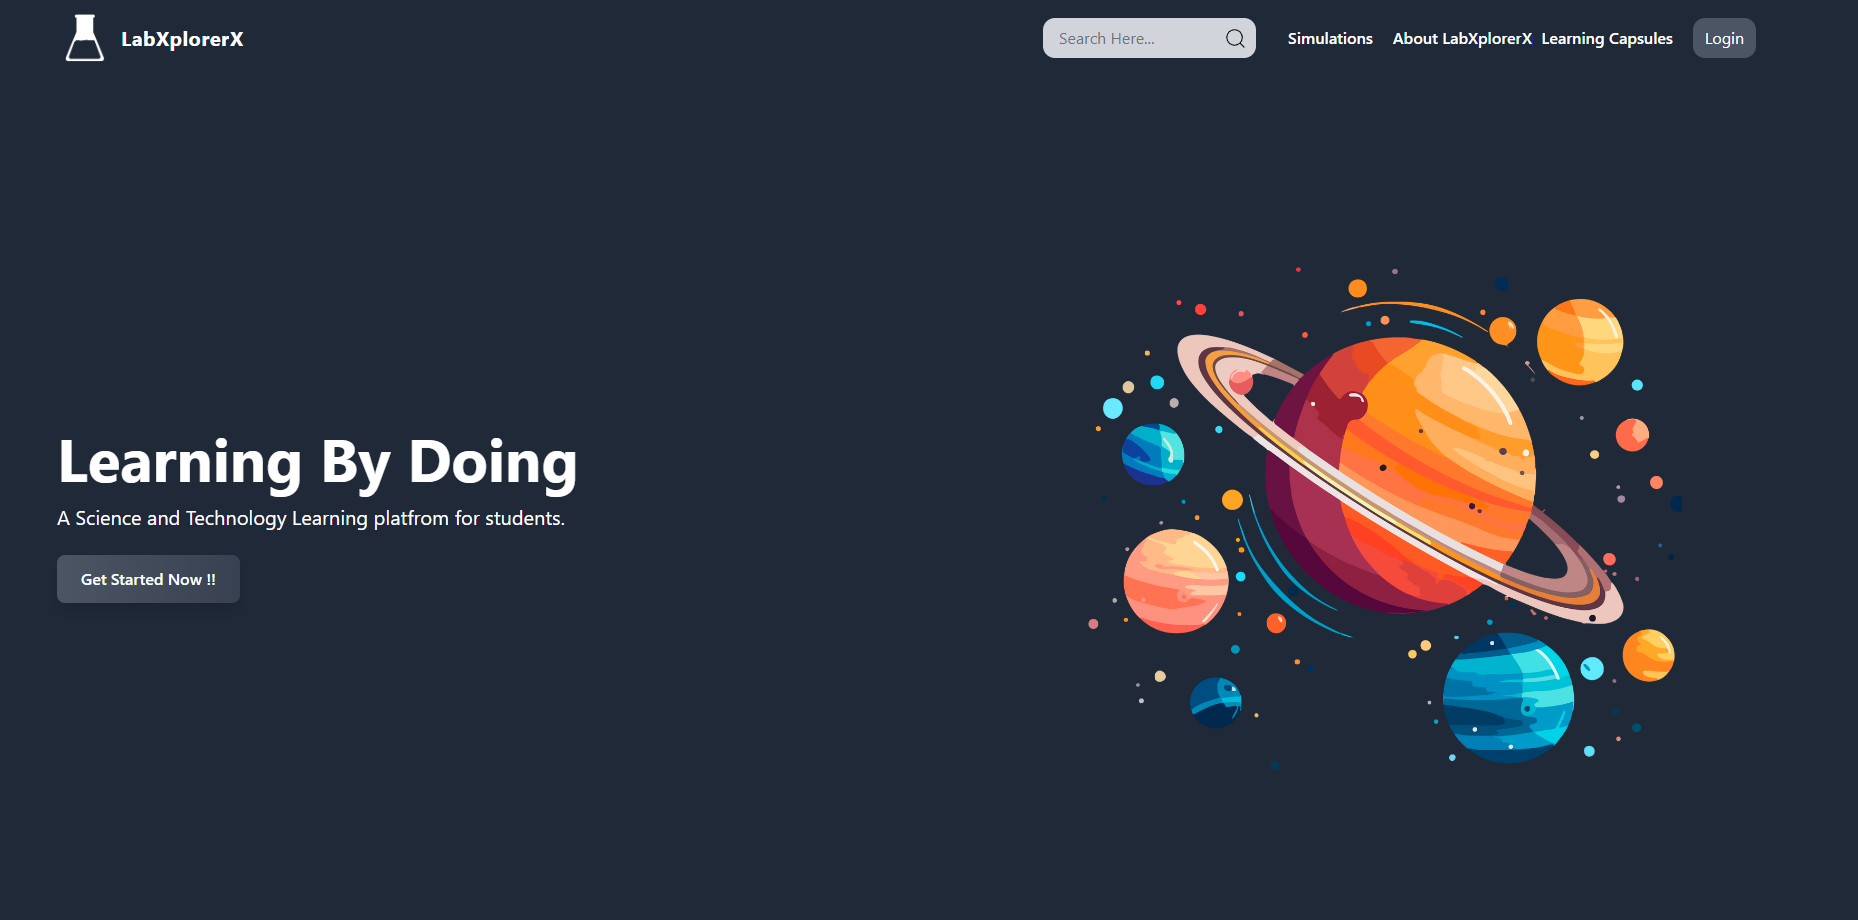
\includegraphics[width = 15cm]{Diagrams/interface/home ui.png}
    \caption{Home Screen UI Design}
\end{figure}
\begin{figure}[H]
    \centering
     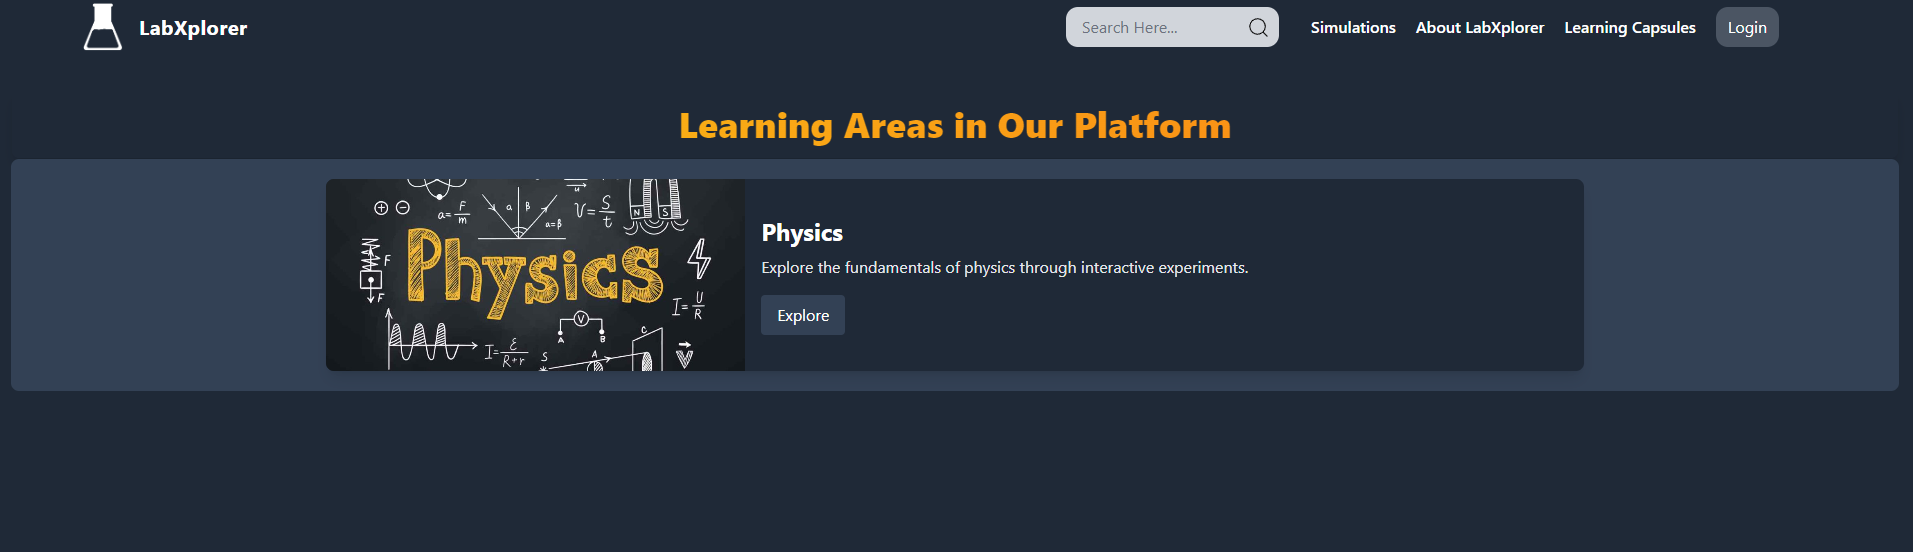
\includegraphics[width = 15cm]{Diagrams/interface/capsule category ui.png}
     \caption{Capsule Category UI Design}
 \end{figure}
 \begin{figure}[H]
    \centering
     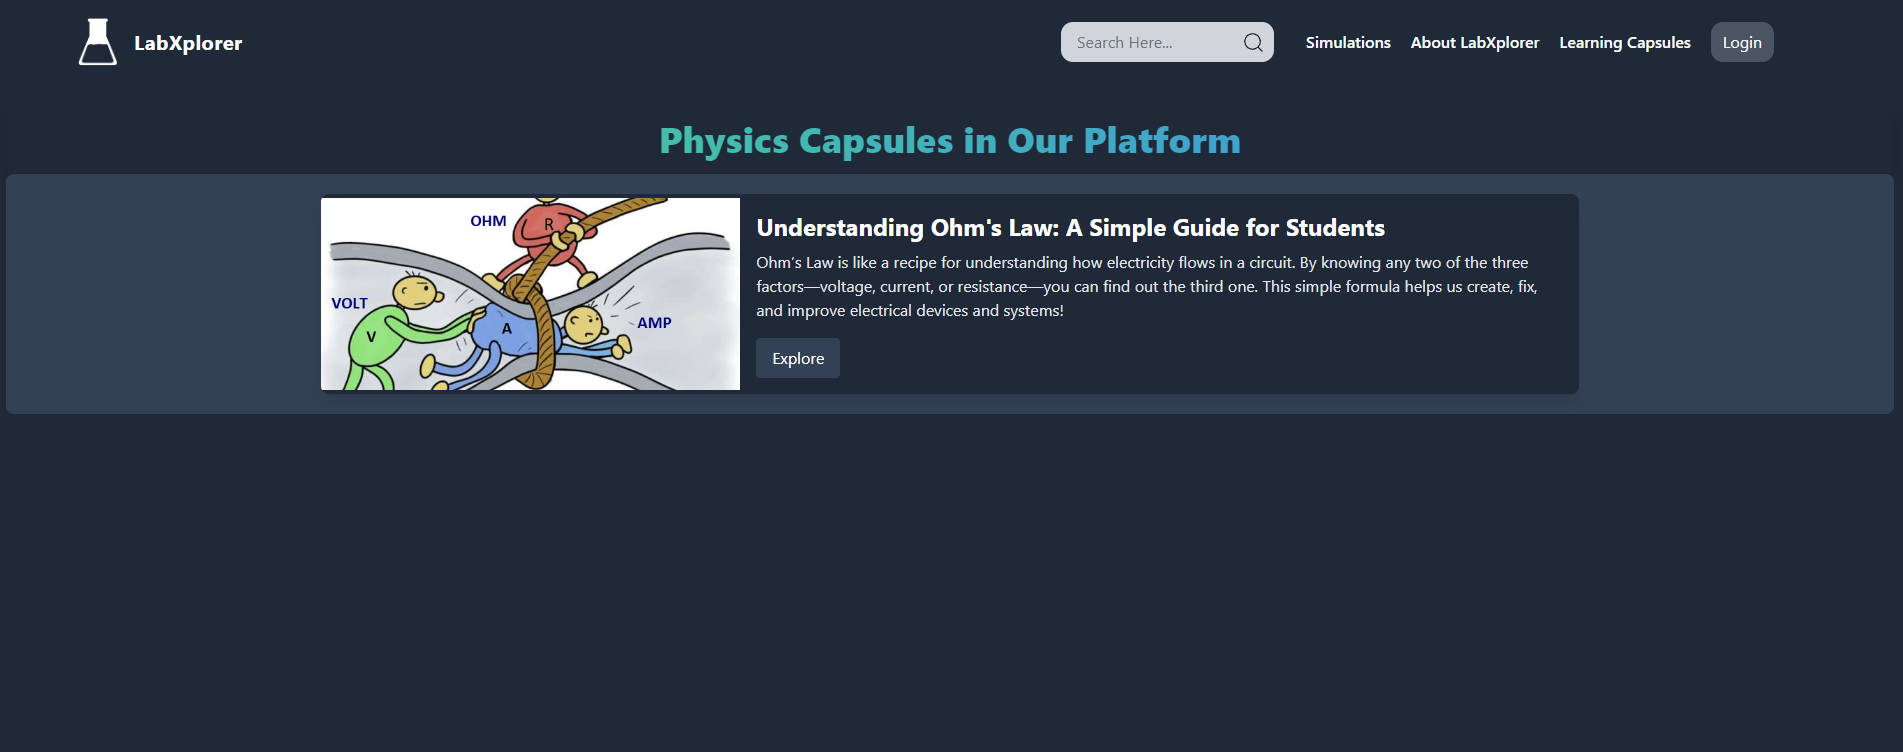
\includegraphics[width = 15cm]{Diagrams/interface/Capsules.png}
     \caption{Capsules Menu Design}
 \end{figure}
\newpage
\subsection{Physical DFD}
This Physical Data Flow Diagram (DFD) outlines the architecture of a web application with a clear separation of frontend and backend components. On the backend, Express (Node.js) handles the server-side logic, with middleware for authentication and error handling, routes for user, admin, and capsules, asynchronous controllers for managing requests, and a PostgreSQL database for storing data. Static files, including Unity simulations, are served from the backend. The frontend is built with React.js, utilizing React Router for navigation and RTK slices and APIs for state management. Screens and UI components, along with Phaser simulations, allow users to interact with backend data and display both static and dynamic simulations. The central store handles state management locally across components.
\begin{figure}[H]
    \centering
    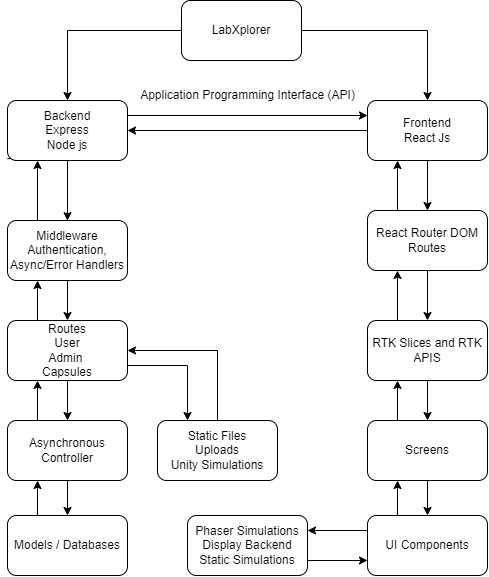
\includegraphics[height = 14cm]{Diagrams/DFD Process Modeling.png}
    \caption{Process Modelling}
\end{figure}

% \section{Algorithm Details}